\chapter{Specific requirements}
	\section{External Interface Requirements}
		\subsection{User Interfaces}
		\subsection{Hardware Interfaces}
			There are no specific hardware interfaces required, except for the devices used to access the platform. Both students and companies need a hardware device (such as a computer) with a network card to connect to S\&C.
		\subsection{Software Interfaces}
				To manage the sending of all notifications (recommendation notifications, notifications for selection results, etc.) between two or more users, the \textit{mail service} must be used. In fact, both students and companies are required to provide their email address (university/company email) during registration. Every time the system sends a notification to a user, they will receive an email informing them of the received notification. To view the content of the notification in more detail, the user must log into the system and go to the appropriate section of the platform.
				
				To do this, the system will send a request to the mail service, which will then forward the desired email to the specific user.
		\subsection{Communication Interfaces}
			Both students and companies use the Internet to access the platform; in particular, companies require an Internet connection for all the functionalities they can perform through the platform (posting internship advice, configuring the selection process, etc.). Similarly, students also need an Internet connection for their functionalities (searching for internships, applying, etc.).
			
			Due to the confidentiality of exchanged data, a secure communication mean is required, such as HTTPS or VPN.
	\section{Functional Requirements (and goals mapping)}
		Here are described all the functional requirements of the S\&C platform.
		
		\subsection{General requirements}
		
		[R00000] when a notification of a user is generated, the user receives it on its mailbox (in a more concise version) and can consult it on its notification section
		
		\subsection{Requirements related to goal G1}
		
		[R10101] the system allows students to sign up to the platform with their institutional mails
		
		[R10102] the system allows a student to set up whether he/she wants to take part into the recommendation
		
		[R10103] the system allows students upload their CV to the platform
		
		[R10104] the system allows students to publish on their profile a brief description of themselves
		
		[R10105] the system allows students to log in into the system by providing the registration mail and the chosen	password
		
		[R10106] the system allows students to change their profile information (including the CV) and their access information
		
		[R10107] when a student registers, the system extracts from the CV name and surname to create the profile
		
		[R10201] the system allows companies to sign up to the platform with their company address
		
		[R10202] the system allows companies to insert the main information regarding their business area and area of expertise
		
		[R10203] the system allows a company to set up if it wants to take part into the recommendation analysis
		
		[R10204] the system allows companies to log in into the system by providing the registration mail and the chosen password
		
		[R10205] the system allows companies to change their profile information and their access information
		
		[R10301] the system allows companies to publish internship advice where they specify the main information regarding the internship (brief description, experience required, desired skills, main activities involved and the terms) and the submission deadline
		
		[R10302] the system allows companies to delete internship advice which deadline is not expired yet
		
		[R10401] the system allows students to search internships advice by name The system shall act as a search engine to present also the names of the advice that are similar to the searched one
		
		[R10402] the system allows students to search companies by name (and also to see the complete list of registered companies) and then access to their profile
		
		[R10403] the system allows students to filter the results they searched (e.g. ”only paid internships”, ”only companies located in Lombardy”)
		
		[R10404] the system allows students to consult the list of all published internship advice, listed from the most recent to the last
		
		[R10501] when the system recognizes that a new internship advice that might interest a student (that allowed the recommendation option) published, it notifies that student
		
		[R10601] when the system recognizes that a student has a profile that would fit an internship advice, the company that published the advice is notified (for students and companies that both take part into the recommendation analysis)
		
		[R10701] the system allows students to apply for any internship advice which deadline has not expired
		
		[R10702] when a student applies for an internship, the related company is notified by the system
		
		[R10801] the system allows companies to approve, discard or ignore each application they may receive for one of their published advice
		
		[R10901] when a company opens a student profile, it can propose to him to apply for one of its internships. Then, the students receives a notification
		
		[R11001] the system allows student that received an internship proposal from a company can decide to accept it, discard it or ignore it
		
		[R11002] when a student accept an internship proposal, it is implicitly accepted by the company 
		
		[R11101] when a student gets his/her result of the selection, the system provides to him a non-compulsory questionnaire regarding his/her experience (in the context of that selection process)
		
		[R11102] when a company ends a selection process, the system provides to it a non-compulsory questionnaire regarding its experience (in the context of that selection process) 
		
		[R11201] when a student concludes an internship, the system provides to him/her a non-compulsory questionnaire regarding him/her experience (in the context of that internship) and in the meantime it provides to the internship company an analogue questionnaire also non-compulsory 
		
		\subsection{Requirements related to goal G2}
		
		[R20101] when the deadline for an internship advice is expired, the system allows the company to set up the selection process by specifying for each step, the relative questionnaire (with metrics for each question) and the date in which provide it to a student (dates may differ between different students)
		
		[R20102] the system includes into a selection process only student that had an accepted application for the relative internship advice
		
		[R20201] the system notifies students for any interview date that interest them
		
		[R20202] the system allows companies insert students answers into the system
		
		[R20203] the system automatically calculates the scores of questionnaire closed answers
		
		[R20204] the system allows companies to manually insert scores for questionnaire open answers
		
		[R20205] the system allows companies to visualize and compare selections scores
		
		[R20206] in any selection phase, the system allows companies to discard a student currently involved in the selection process (discarded students are removed by the selection process)
		
		[R20207] in any selection phase, the system allows companies to accept a student currently involved in the selection process (accepted students are removed by the selection process)
		
		[R20208] the system allows companies to write a personalized message to communicate the result of a selection
		
		[R20209] when a selection result is prepared for a student (with the relative message), it is notified to the student
		
		[R20210] when a selected process related to an internship advice has ended, the system deletes the advice
		
		\subsection{Requirements related to goal G3}
		
		[R30101] the system allows students and companies to consult the internships (ongoing or finished)
		
		[R30102] the system allows students and companies to report complaints (at most 50 words)on the internships they are involved in
		
		[R30103] the system does not allow users different from their creator to consult complains
		
		[R30104] when an ongoing internship finishes (ending date is reached), involved users are notified and the system still permits users to see it but marks it as "closed"
		
		[R30105] the system allows companies to manually close their ongoing internships (each one) before the closing deadline
		
		\subsection{Use-case diagram}
			
			\begin{figure}[H]
				\centering
				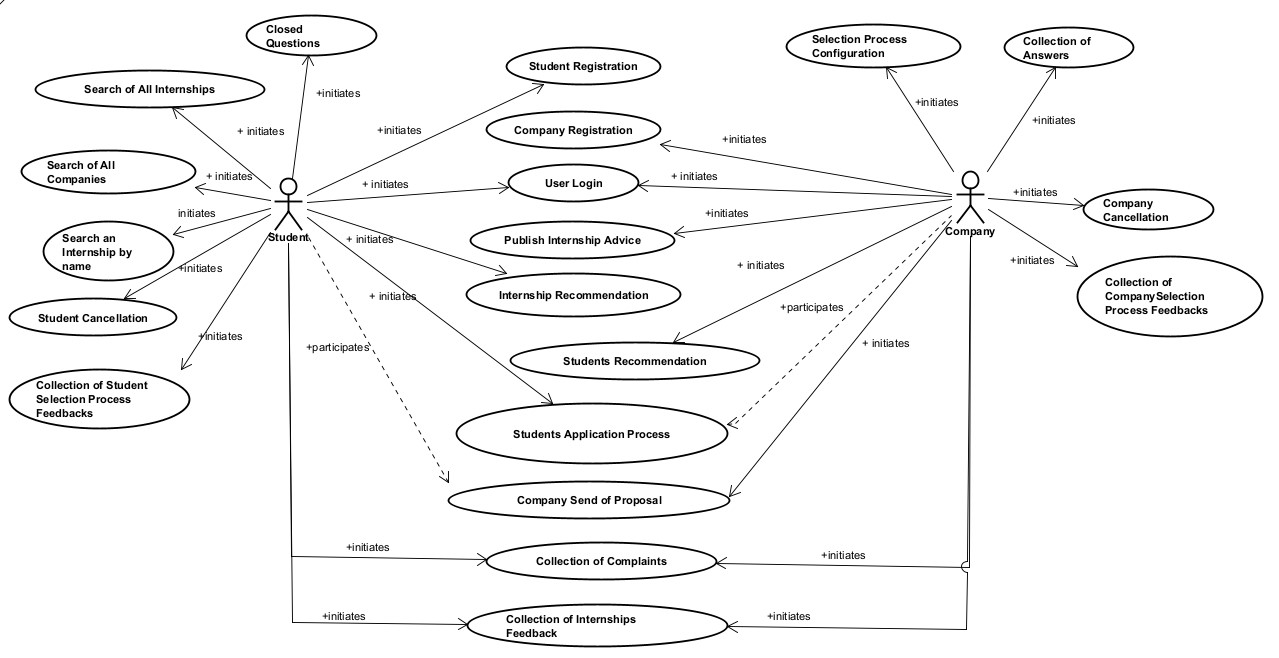
\includegraphics[scale=1.0]{UC.jpg}
				\caption{Use-case diagram}
			\end{figure}
			
			The Use Case (UC) diagram shows, for each defined UC, which actors are involved and, in general, which actor initiates the UC. For UCs that can be performed by both actors (students and companies), the common name \textit{User} is used.	
			
		\subsection{Use-cases}
			
			\begin{table} [H]
				\centering
				\begin{itemize}
					\item [UC1] - Student Registration
				\end{itemize}
				\begin{tabular}{|| P{7.5cm} | P{7.5cm} ||}
					\hline
					Name & Student Registration \\
					\hline
					Actors & \parbox{5cm}{\begin{itemize}
							\item Student
							\end{itemize}
						} \\
					\hline
					Entry condition & The student has opened the S\&C platform for the first time \\
					\hline
					Event Flow & \parbox{5cm}{\begin{enumerate}
						\item The student press the button \textit{Registration}
						\item The student press the button \textit{Student Registration}
						\item The system shows a form to compile
						\item The Student compile the form providing his institutional e-mail and password and a brief description on his academic 
						background
						\item The Student flags the \textit{receive 
						notification} box (part of the form) 
						if he wants to take part into the recommendation process 
						\item The student press the button 
						\textit{Upload CV} to upload the 
						curriculum (the button is part of 
						the form)
						\item The student press the button 
						\textit{Register} to complete the 
						registration
						\item the system checks the digital signature on the CV
						\end{enumerate}} \\
					\hline 
					Exit condition & The student has successfully registered 
					to the platform and the system shows the 
					homepage \\
					\hline
					Exception & There already exist a student with those e-mail; the system return to the entry condition showing an error message \textit{Student already registered} \\
					\hline
				\end{tabular}
			\end{table}
			
			
		
			
			\begin{table} [H]
				\centering
					\begin{itemize}
					\item [UC2] - Company Registration
				\end{itemize}
				\begin{tabular}{|| P{7.5cm} | P{7.5cm} ||}
					\hline
					Name & Company Registration \\
					\hline
					Actors & \parbox{5cm}{\begin{itemize}
							\item Company
						\end{itemize}
					} \\
					\hline
					Entry condition & The company has opened the S\&C platform for the first time \\
					\hline
					Event Flow & \parbox{5cm}{\begin{enumerate}
							\item The company press the button \textit{Registration}
							\item The company press the button \textit{Company Registration}
							\item The system shows a form to compile
							\item The Company compile the form 
							providing its name, a brief description 
							of its area of expertise and business 
							area, its e-mail and password
							\item The Company flags the “receive 
							notification” box (part of the form) if it 
							wants to take part into the recommendation process
							\item The company press the button 
							\textit{Register} to complete the 
							registration
					\end{enumerate}} \\
					\hline 
					Exit condition & The company has successfully registered 
					to the platform and the system shows the 
					homepage \\
					\hline
					Exception & There arleady exist a company with 
					those e-mail; the system return to 
					the entry condition showing an 
					error message \textit{Company arleady 
						registered} \\
					\hline
				\end{tabular}
			\end{table}
			
		
			
			\begin{table} [H]
				\centering
					\begin{itemize}
					\item [UC3] - User Login
				\end{itemize}
				\begin{tabular}{|| P{7.5cm} | P{7.5cm} ||}
					\hline
					Name & User Login \\
					\hline
					Actors & \parbox{5cm}{\begin{itemize}
							\item User
						\end{itemize}
					} \\
					\hline
					Entry condition & The User has opened the S\&C platform \\
					\hline
					Event Flow & \parbox{5cm}{\begin{enumerate}
							\item The user press the button \textit{Login}
							\item The system shows the Login page
							\item The user logged to the platform 
							inserting e-mail and password 
							\item The user press the button \textit{Log}
					\end{enumerate}} \\
					\hline 
					Exit condition & the user has successfully logged to the 
					platform and the homepage is shown \\
					\hline
					Exception & \parbox{5cm}{\begin{enumerate}
							\item The user has not yet registered to the 
							platform; the system will return to the 
							registration page
							\item the credentials are not correct; the system shows an error message and the system return to the login page
							\end{enumerate}} \\
					\hline
				\end{tabular}
			\end{table}
			
		
			
			\begin{table} [H]
				\centering
					\begin{itemize}
					\item [UC4] - Publish Internship Advice
				\end{itemize}
				\begin{tabular}{|| P{7.5cm} | P{7.5cm} ||}
					\hline
					Name & Publish Internship Advice \\
					\hline
					Actors & \parbox{5cm}{\begin{itemize}
							\item Company
						\end{itemize}
					} \\
					\hline
					Entry condition & The company is logged to S\&C platform and it wants to publish a new internship advice \\
					\hline
					Event Flow & \parbox{5cm}{\begin{enumerate}
							\item The company goes to the \textit{Publish 
							New Internship} section
							\item The company press the button \textit{Add 
							New Internship Advice} 
							\item The system shows a form to compile
							\item The company compile the form by 
							providing: the title, the subject, a 
							brief description of the internship, 
							experience required and desired 
							skills, the main activities the 
							internship involved, the terms of the 
							offer, the advice deadline and the 
							max number of applications
							\item The company press the button 
							\textit{Publish}
					\end{enumerate}} \\
					\hline 
					Exit condition & The company has successfully published a 
					new internship advice and the system 
					return to the homepage  \\
					\hline
					Exception & The company doesn’t fill all the 
					fields of the form; the system will 
					warn the company \\
					\hline
				\end{tabular}
				\end{table}
				
				
				
				\begin{table} [H]
					\centering
					\begin{itemize}
						\item [UC5] - Search of all Internships
					\end{itemize}
					\begin{tabular}{|| P{7.5cm} | P{7.5cm} ||}
						\hline
						Name & Search of All Internships \\
						\hline
						Actors & \parbox{5cm}{\begin{itemize}
								\item Student
							\end{itemize}
						} \\
						\hline
						Entry condition & The student is logged to S\&C platform and he wants to apply for an internship  \\
						\hline
						Event Flow & \parbox{5cm}{\begin{enumerate}
								\item The student goes to the \textit{View 
									Internships} section
								\item The system shows the page with a 
								list of all the published internships advice, 
								listed from the most recent to the 
								last recent  
								\item The student select an internship advice who interested them
						\end{enumerate}} \\
						\hline 
						Exit condition &  the system shows the 
						page with all the details about the 
						internship \\
						\hline
						Exception & The student doesn’t find an interesting 
						internship; in this case he returns to the 
						home page clicking on the button \textit{Home}
						the system returns to the homepage 
						 \\
						\hline
					\end{tabular}
				\end{table}
				
				
				
				
				\begin{table} [H]
					\centering
					\begin{itemize}
						\item [UC6] - Search of all Companies
					\end{itemize}
					\begin{tabular}{|| P{7.5cm} | P{7.5cm} ||}
						\hline
						Name & Search of all Companies \\
						\hline
						Actors & \parbox{5cm}{\begin{itemize}
								\item Student
							\end{itemize}
						} \\
						\hline
						Entry condition & The student is logged to S\&C platform and he wants to apply for an internship \\
						\hline
						Event Flow & \parbox{5cm}{\begin{enumerate}
								\item The student goes to the \textit{View 
									Companies} section
								\item The system shows the page with a 
								list of all the company registered to 
								the sytem, listed in alphabetical 
								order   
								\item The student clicks on the name of 
								the company who interested him
								\item The system shows the list of all 
								internships advices published by 
								the company 
								\item The student select an internship advice who 
								interested them
						\end{enumerate}} \\
						\hline 
						Exit condition &  the system shows the 
						page with all the details about the 
						internship \\
						\hline
						Exception & The student doesn’t find an interesting 
						internship; in this case he returns to the 
						home page clicking on the button \textit{Home}
						the system returns to the homepage 
						\\
						\hline
					\end{tabular}
				\end{table}
				
				
				
				\begin{table} [H]
					\centering
					\begin{itemize}
						\item [UC7] - Search an internship by name 
					\end{itemize}
					\begin{tabular}{|| P{7.5cm} | P{7.5cm} ||}
						\hline
						Name & -Search an internship by name \\
						\hline
						Actors & \parbox{5cm}{\begin{itemize}
								\item Student
							\end{itemize}
						} \\
						\hline
						Entry condition & The student is logged to S\&C platform and he wants to apply for an internship \\
						\hline
						Event Flow & \parbox{5cm}{\begin{enumerate}
								\item The student search the internship 
								by typing its subject on the search 
								bar 
								\item The student flags the appropriate 
								options they want the internship to 
								meet  
								\item The systems shows a page with all 
								the internships advice matching 
								the subject and the options chosen, from the most relevant from the last
								\item The student select an internship who 
								interested them
						\end{enumerate}} \\
						\hline 
						Exit condition &  the system shows the 
						page with all the details about the 
						internship \\
						\hline
						Exception & \parbox{5cm}{\begin{enumerate}
								\item The student digits a subject and no 
								internships match it. The system 
								will warn the student that no 
								internships are found 
								\item The student doesn’t find an 
								interesting internship; in this case 
								he returns to the home page 
								clicking on the button \textit{Home}; the 
								system returns to the homepage
								\end{enumerate}} \\
						\hline
					\end{tabular}
				\end{table}
				
				
					
				
				\begin{table} [H]
					\centering
					\begin{itemize}
						\item [UC8] - Internship Recommendation
					\end{itemize}
					\begin{tabular}{|| P{7.5cm} | P{7.5cm} ||}
						\hline
						Name & Internship Reccomendation \\
						\hline
						Actors & \parbox{5cm}{\begin{itemize}
								\item Student
							\end{itemize}
						} \\
						\hline
						Entry condition & the student, at registration, flags the 
						option to receive notifications and the recommendation analysis is completed\\
						\hline
						Event Flow & \parbox{5cm}{\begin{enumerate}
								\item The student logs to the platform  
								\item the student goes to the \textit{Notification} 
								section
								\item  the student clicks on the notification 
								related to the new internship 
								published
								\item the system shows the page with the 
								details about the internship  
						\end{enumerate}} \\
						\hline 
						Exit condition & The student view the internship more in 
						detail \\
						\hline
					\end{tabular}
				\end{table}
				
				\begin{table} [H]
					\centering
					\begin{itemize}
						\item [UC9] - Students Recommendation
					\end{itemize}
					\begin{tabular}{|| P{7.5cm} | P{7.5cm} ||}
						\hline
						Name & Students Recommendation \\
						\hline
						Actors & \parbox{5cm}{\begin{itemize}
								\item Company
							\end{itemize}
						} \\
						\hline
						Entry condition & the company, at registration, flags the 
						option to receive notifications and the recommendation analysis is completed\\
						\hline
						Event Flow & \parbox{5cm}{\begin{enumerate}
								\item The comapny logs to the platform  
								\item the company goes to the \textit{Personal Internships} 
								section
								\item  the company clicks on the internship related to the notification
								\item the company goes on the \textit{Notification} section 
								\item the system shows the page with all the notification related to the internship
								\item the company select the notification it has to consider
								\item the system shows the notification with the list of the name of the students
								\item the company clicks on one of the name
						\end{enumerate}} \\
						\hline 
						Exit condition & The company view the profile of the student more in 
						detail \\
						\hline
					\end{tabular}
				\end{table}
				
				
			
				
				\begin{table} [H]
					\centering
						\begin{itemize}
						\item [UC10] - Students Application Process
					\end{itemize}
					\begin{tabular}{|| P{7.5cm} | P{7.5cm} ||}
						\hline
						Name & Students Application process \\
						\hline
						Actors & \parbox{5cm}{\begin{itemize}
								\item Student
								\item Company
							\end{itemize}
						} \\
						\hline
						Entry condition & the student is logged to S\&C platform and he finds an internship he wants to apply \\
						\hline
						Event Flow & \parbox{5cm}{\begin{enumerate}
								\item The student access the page of the 
								internship he wants to apply (in any way) 
								\item The system shows the page of the 
								internship 
								\item The student click on \textit{Apply} button
								\item  The system sends an e-mail to the 
								company providing the internship
								\item The company logs to the system with 
								its credentials
								\item The company goes to \textit{Personal 
								Internships} section
								\item The company select the 
								corresponding internship
								\item The company goes to \textit{Notification} 
								section 
								\item The system shows all the notification 
								of the corresponding internship
								\item The company select the notification 
								of the student 
								\item The company click on \textit{Accept 
								Application} or\textit{Reject Application}
								button to approve or reject the 
								application
						\end{enumerate}} \\
						\hline 
						Exit condition & the system automatically sends an e-mail to 
						the student to to inform whether the 
						application has been accepted or rejected  \\
						\hline
						Exception & The deadline has already passed; the system notifies the student that they cannot apply for that internship \\
						\hline
					\end{tabular}
				\end{table}
				
				
			
				
				\begin{table} [H]
					\centering
						\begin{itemize}
						\item [UC11] - Company Send of Proposal
					\end{itemize}
					\begin{tabular}{|| P{7.5cm} | P{7.5cm} ||}
						\hline
						Name & Company Send of Proposal \\
						\hline
						Actors & \parbox{5cm}{\begin{itemize}
								\item Student
								\item Company
							\end{itemize}
						} \\
						\hline
						Entry condition & the company is logged to S\&C platform and it already received some student through the recommendation mechanism \\
						\hline
						Event Flow & \parbox{5cm}{\begin{enumerate}
								\item the company goes to \textit{Personal Internships} section
								\item the company select the corresponding internship 
								\item the company select a student for that internship
								\item the system shows the profile of the student
								\item the company clicks on "Send Proposal" button
								\item the system sends an email to the student
								\item the student logs into the platform using his credentials
								\item The student goes to \textit{Notification} 
								section 
								\item the student clicks on the notification 
								received 
								\item The student clicks on \textit{Accept 
									Proposal} or\textit{Reject Proposal}
								button to approve or reject the 
								proposal
						\end{enumerate}} \\
						\hline 
						Exit condition & the system return to the homepage \\
						\hline
						Exception & The student respond to the proposal when the deadline has already passed; the 
								system notifies the student that they 
								cannot reply to the proposal \\
						\hline
					\end{tabular}
				\end{table}
				
				
				\begin{table} [H]
					\centering
					\begin{itemize}
						\item [UC12] - Selection Process Configuration
					\end{itemize}
					\begin{tabular}{|| P{7.5cm} | P{7.5cm} ||}
						\hline
						Name & Selection Process Configuration \\
						\hline
						Actors & \parbox{5cm}{\begin{itemize}
								\item Company
							\end{itemize}
						} \\
						\hline
						Entry condition & Internship deadline is expired and the 
						company is logged to S\&C platform  \\
						\hline
						Event Flow & \parbox{5cm}{\begin{enumerate}
								\item The company goes to \textit{Personal 
								Internships} section
								\item The company select the 
								appropriate Internship advice  
								\item The system shows the internship 
								advice page
								\item  The company goes on 
								\textit{Configuration} section
								\item  the company configures the 
								number of steps (up to 2), the 
								metrics to evaluate students and 
								the questionnaire provided at 
								each step (it is defined the structure, deciding which questions are closed or open/oral, and also the score for each closed question)
								\item the company save the 
								configuration clicking on \textit{Save}
								button 
								\item the company goes on \textit{Students 
								Applied} section
								\item the system shows a page with all 
								the students applied for the 
								internship 
								\item the company decided, for each 
								candidate, the date of each step
								\item the company click on the button 
								\textit{Save}
						\end{enumerate}} \\
						\hline 
						Exit condition & The selection process is now configured 
						for each student; the system 
						automatically sends an e-mail to the 
						students to inform them   \\
						\hline
						Exception & \parbox{5cm}{\begin{enumerate}
								\item the company has not configured 
								every part; the system warn the 
								company
								\item The company has not assigned 
								the respective dates for each 
								student \\
						\end{enumerate}} \\
						\hline
					\end{tabular}
				\end{table}
				
				
				\begin{table} [H]
					\centering
					\begin{itemize}
						\item [UC13] - Selection Process Running
					\end{itemize}
					\begin{tabular}{|| P{7.5cm} | P{7.5cm} ||}
						\hline
						Name & Selection Process Running \\
						\hline
						Actors & \parbox{5cm}{\begin{itemize}
								\item Student
								\item Company
							\end{itemize}
						} \\
						\hline
						Entry condition & Internship deadline is expired, the company configure the selection process and it has ready to start \\
						\hline
						Event Flow & \parbox{5cm}{\begin{enumerate}
								\item The company gives to the student the questionnaire with closed and open questions
								\item The student answers to the questionnaire
								\item The company asks some oral questions (if they are configured in this step)
								\item The student answers to oral questions
								\item The company logs to the platform 
								\item the company goes into \textit{Personal Internship} section
								\item the system shows the page with all the personal internships of the company
								\item the company select the appropriate internship 
								\item the company select, from the list of students, the appropriate student
								\item the company select the appropriate step of the selection process
								\item the company click the button \textit{Insert Answers}
								\item the system shows a form to fill with the answers
								\item the company insert the answers
								\item the company clicks on the button \textit{Evaluate}
								\item the system shows the page with the evaluated answers
								\item the company decide to accept/reject/postpone the student
								\item the company click on the appropriate button to send the rigth notification
						\end{enumerate}} \\
						\hline 
						Exit condition & the evaluation of this step of the selection process is completed; the system send a notification to the student to inform him about the decision of the company   \\
						\hline
						Exception & the company doesn't insert all the answers; the system shows an error message and the company has to fill all the fields of the form \\
						\hline
					\end{tabular}
				\end{table}
				
				
				\begin{table} [H]
					\centering
					\begin{itemize}
						\item [UC14] - Collection of Student Selection Process Feedback
					\end{itemize}
					
					\begin{tabular}{|| P{7.5cm} | P{7.5cm} ||}
						\hline
						Name & Collection of Student Selection Process Feedback \\
						\hline
						Actors & \parbox{5cm}{\begin{itemize}
								\item Student
							\end{itemize}
						} \\
						\hline
						Entry condition & the selection process is complete and the student has already received the email with the result of the interview \\
						\hline
						Event Flow & \parbox{5cm}{\begin{enumerate}
								\item The student logs into the platform with his credentials
								\item The student goes to the \textit{Notification} Section
								\item The system shows the page with all the notifications for the student
								\item The student open the notification related to the selection process result 
								\item The student open the questionnaire attached to the notification
								\item The system shows a form with a series of questions to answer
								\item The student answers to the questions 
								\item The student clicks the button \textit{Submit} to submit the feedback
						\end{enumerate}} \\
						\hline 
						Exit condition & the feedback is submitted; the system collects the feedback in order to improve the recommendation 
						mechanism \\
						\hline
						Exception & the student doesn't answer to all the questions when he tries to submit; the system shows a warn message \\
						\hline
					\end{tabular}
				\end{table}
				
				\begin{table} [H]
					\centering
					\begin{itemize}
						\item [UC15] - Collection of Company Selection Process Feedback
					\end{itemize}
					
					\begin{tabular}{|| P{7.5cm} | P{7.5cm} ||}
						\hline
						Name & Collection of Company Selection Process Feedback \\
						\hline
						Actors & \parbox{5cm}{\begin{itemize}
								\item Company
							\end{itemize}
						} \\
						\hline
						Entry condition & The company is logged to S\&C platform and has just sent the selection results \\
						\hline
						Event Flow & \parbox{5cm}{\begin{enumerate}
								\item The system shows a form with a series of questions to answer 
								\item the company answers to the questions
								\item the company clicks on the button \textit{Submit}
						\end{enumerate}} \\
						\hline 
						Exit condition & the feedback is submitted;the system collects the
						feedback in order to improve the recommendation
						mechanism \\
						\hline
						Exception & the company doesn't answer to all the questions when he tries to submit; the system shows a warn message \\
						\hline
					\end{tabular}
				\end{table}
				
						\begin{table} [H]
					\centering
					\begin{itemize}
						\item [UC16] - Collection of Internship Feedback
					\end{itemize}
					
					\begin{tabular}{|| P{7.5cm} | P{7.5cm} ||}
						\hline
						Name & Collection of Internships Feedback \\
						\hline
						Actors & \parbox{5cm}{\begin{itemize}
								\item User
							\end{itemize}
						} \\
						\hline
						Entry condition & The User is logged to S\&C platform and it completed an internship \\
						\hline
						Event Flow & \parbox{5cm}{\begin{enumerate}
								\item The user goes to \textit{Ongoing Internships} section
								\item The system shows a page with 
								all the ongoing internships of the user 
								\item The User select the interested 
								internship  
								\item the User opens the form in the page of the internship
								\item the system shows a form with a series of questions to answer 
								\item the User answers to the questions
								\item the User clicks on the button \textit{Submit}
						\end{enumerate}} \\
						\hline 
						Exit condition & the feedback is submitted;the system collects the
						feedback in order to improve the recommendation
						mechanism \\
						\hline
						Exception & the user doesn't answer to all the questions when he tries to submit; the system shows a warn message \\
						\hline
					\end{tabular}
				\end{table}
				
				
				\begin{table} [H]
					\centering
					\begin{itemize}
						\item [UC17] - Collection of Complaints
					\end{itemize}
					
					\begin{tabular}{|| P{7.5cm} | P{7.5cm} ||}
						\hline
						Name & Collection of Complaints \\
						\hline
						Actors & \parbox{5cm}{\begin{itemize}
								\item User
							\end{itemize}
						} \\
						\hline
						Entry condition & The user is logged to S\&C platform, 
						and there is an ongoing internship in 
						which it is involved.  \\
						\hline
						Event Flow & \parbox{5cm}{\begin{enumerate}
								\item The user goes on \textit{Ongoing 
								Internships} section 
								\item The system shows a page with 
								all the ongoing internships 
								related to the user  
								\item The user select the interested 
								internship  
								\item The system shows the page 
								where the user can monitor the 
								execution of the internship
								\item The user write a complaint 
								using the apposite box (max 50 
								words) 
								\item The user click on the \textit{Submit}
								button
						\end{enumerate}} \\
						\hline 
						Exit condition & The complaint has been submitted; 
						the system collect the complain 
						related to the internship \\
						\hline
						Exception & The complain exceed the max number 
						of words (50); the system warn the 
						user that the complaint is too long \\
						\hline
					\end{tabular}
				\end{table}
				
				
				\begin{table} [H]
					\centering
					\begin{itemize}
						\item [UC18] - Delete Internship Advice
					\end{itemize}
					
					\begin{tabular}{|| P{7.5cm} | P{7.5cm} ||}
						\hline
						Name & Delete Internship advice \\
						\hline
						Actors & \parbox{5cm}{\begin{itemize}
								\item Company
							\end{itemize}
						} \\
						\hline
						Entry condition & the company is logged to the platform, it finished a selection process and it wants to delete and internship advice  \\
						\hline
						Event Flow & \parbox{5cm}{\begin{enumerate}
								\item The company goes on \textit{Personal Internships} section 
								\item The system shows a page with 
								all the internships advice of the company  
								\item The user select the interested 
								internship advice 
								\item The user click on \textit{Delete} button
						\end{enumerate}} \\
						\hline 
					\end{tabular}
				\end{table}
				
		\subsection{Sequence diagrams}
		
			\begin{figure}[H]
				\centering
				{\bfseries [UC1] - Student Registration}
				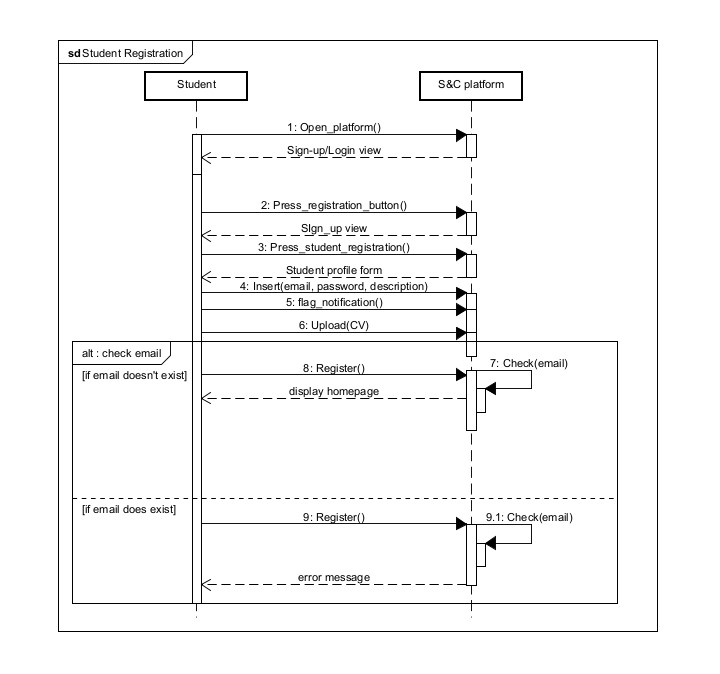
\includegraphics[scale=0.3]{StudentRegistration.jpg}
				\caption{[UC1] - Student Registration}
			\end{figure}
			
			\begin{figure}[H]
				\centering
				{\bfseries [UC2] - Company Registration}
				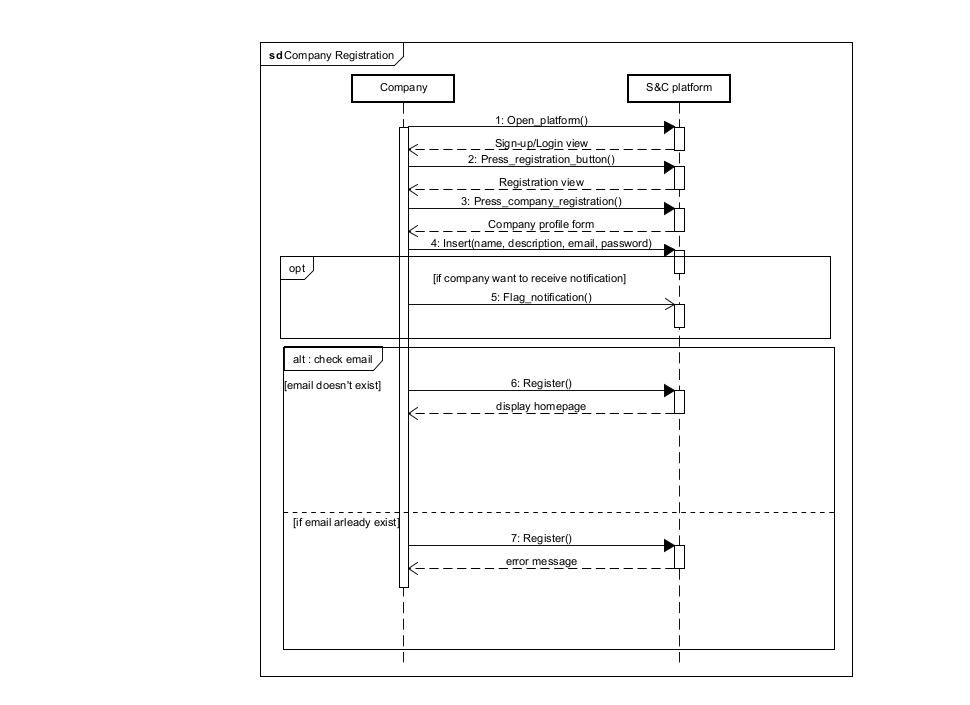
\includegraphics[scale=0.3]{CompanyRegistration.jpg}
				\caption{[UC2] - Company Registration}
				
			\end{figure}
			
			\begin{figure}[H]
				\centering
				{\bfseries [UC3] - User Login}
				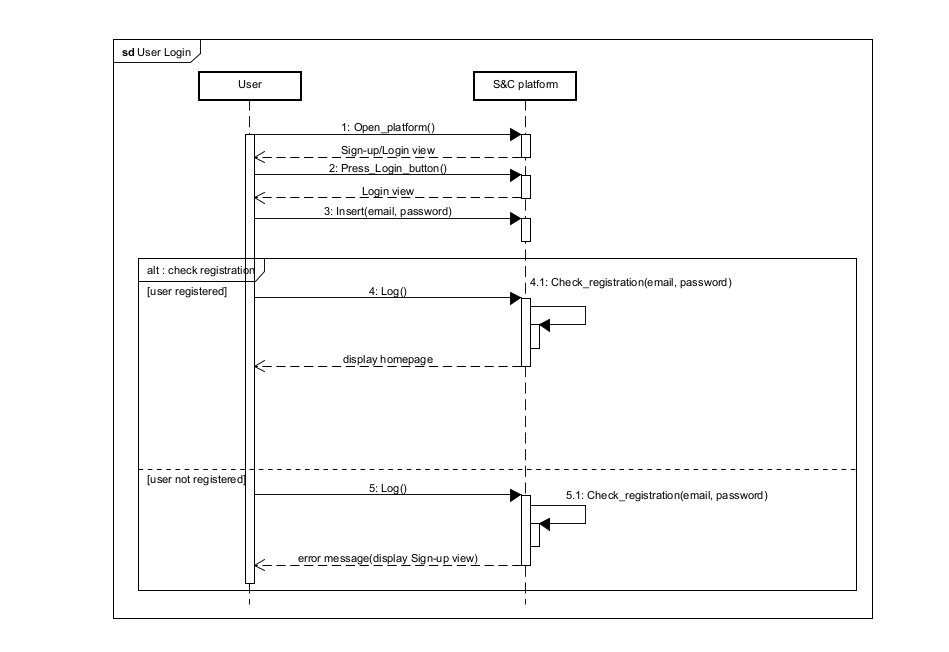
\includegraphics[scale=0.3]{UserLogin.jpg}
				\caption{[UC3] - User Login}
				
			\end{figure}
			
			\begin{figure}[H]
				\centering
				{\bfseries [UC4] - Publish Internship Advice}
				\caption{[UC4] - Publish Internship Advice}
				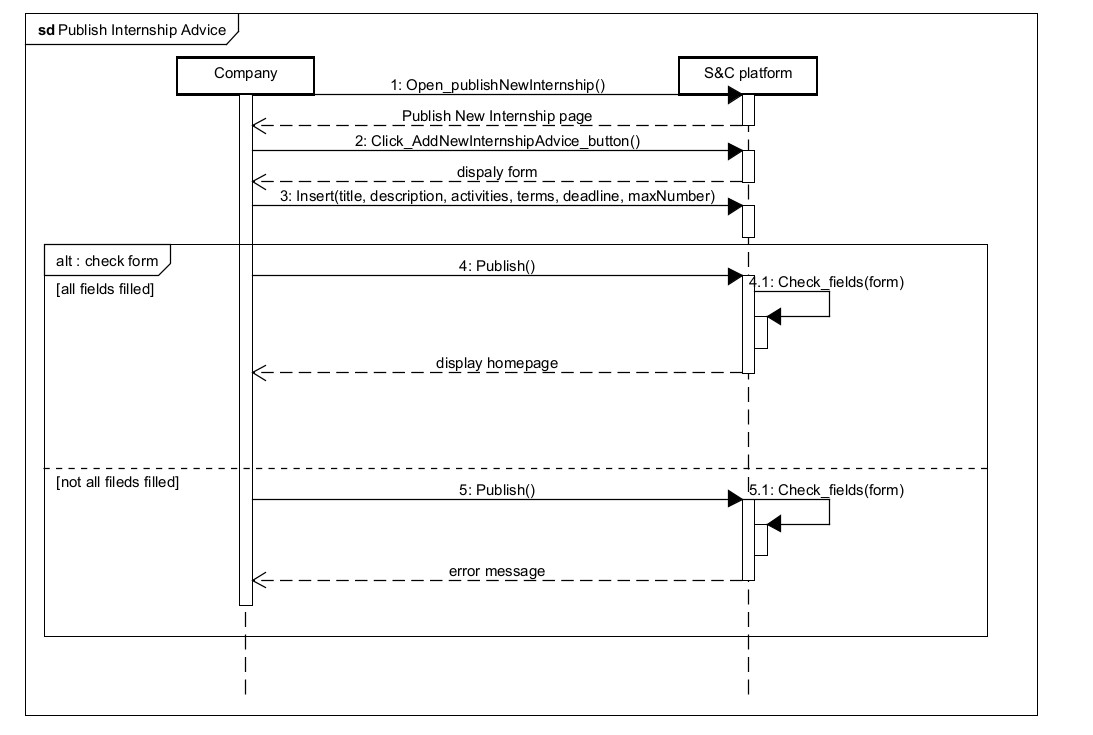
\includegraphics[scale=0.3]{PublishInternshipAdvice.jpg}
				
				
			\end{figure}
			
		
			\begin{figure}[H]
				\centering
				{\bfseries [UC5] - Search of all Internships}
				\caption{[UC5] - Search of all Internships}
				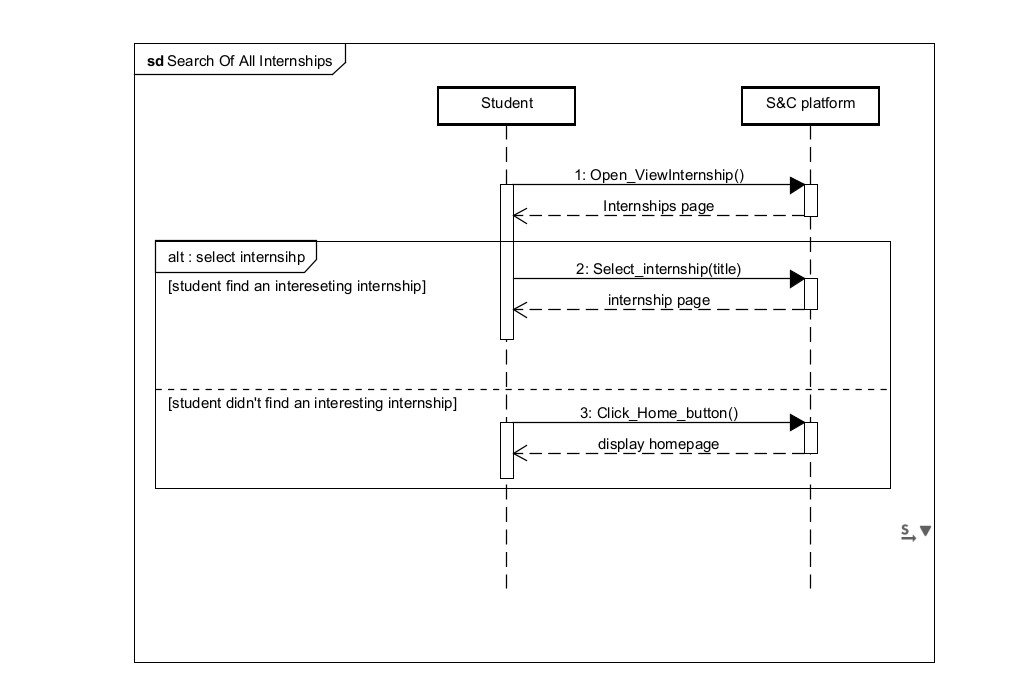
\includegraphics[scale=0.3]{SearchAllInternships.jpg}
				
			\end{figure}
			
			\begin{figure}[H]
				\centering
				{\bfseries [UC6] - Search of All Companies}
				\caption{[UC6] - Search of All Companies}
				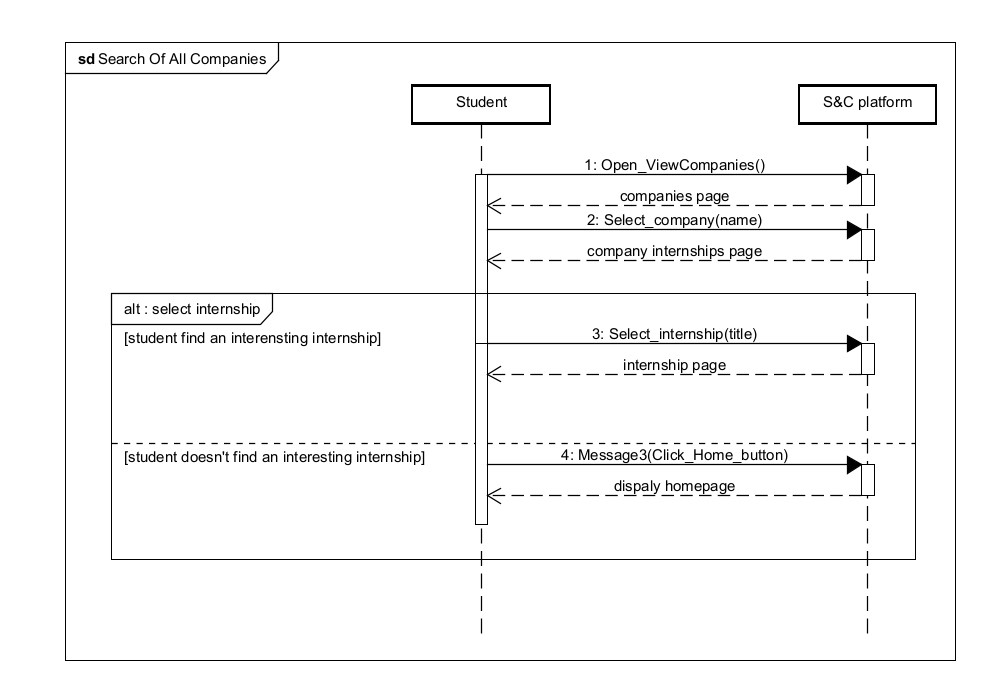
\includegraphics[scale=0.3]{SearchAllCompanies.jpg}
				
			\end{figure}
			
			\begin{figure}[H]
				\centering
				{\bfseries [UC7] - Search an Internship by Name}
				\caption{[UC7] - Search an Internship by Name}
				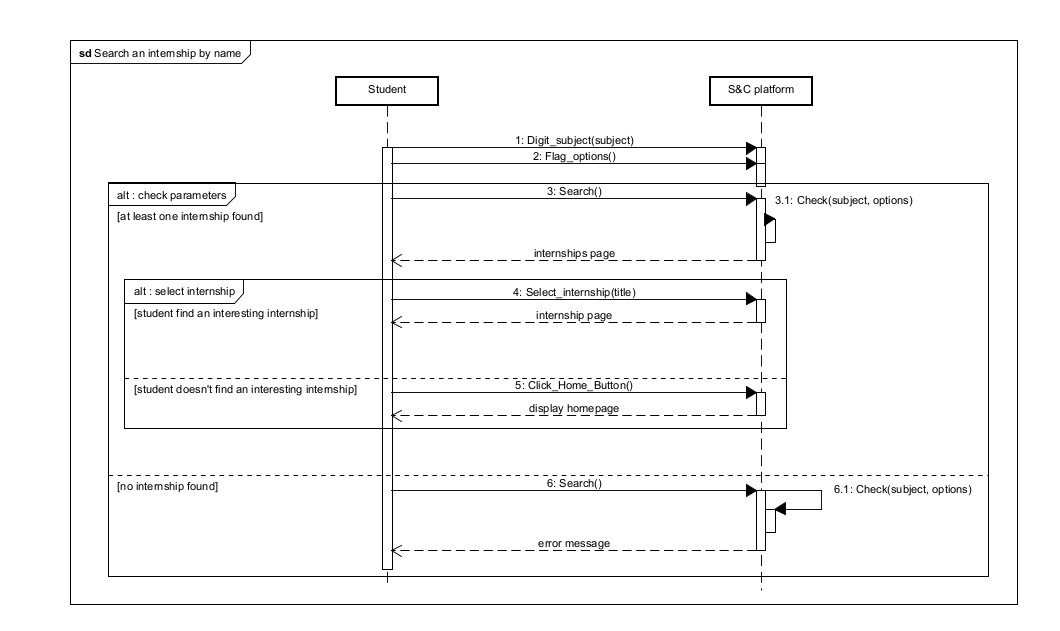
\includegraphics[scale=0.3]{SearchByName.jpg}
				
			\end{figure}
			
			\begin{figure}[H]
				\centering
				{\bfseries [UC8] - Internship Recommendation}
				\caption{[UC8] - Internship Recommendation}
				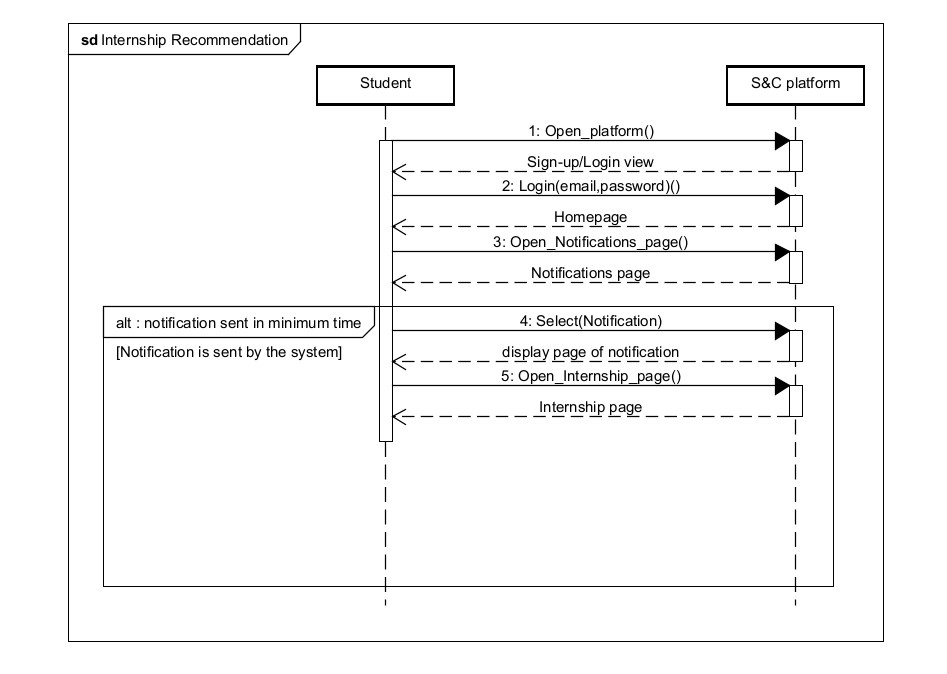
\includegraphics[scale=0.3]{InternshipRecommendation.jpg}
				
			\end{figure}
			
			\begin{figure}[H]
				\centering
				{\bfseries [UC9] - Students Recommendation}
				\caption{[UC9] - Students Recommendation}
				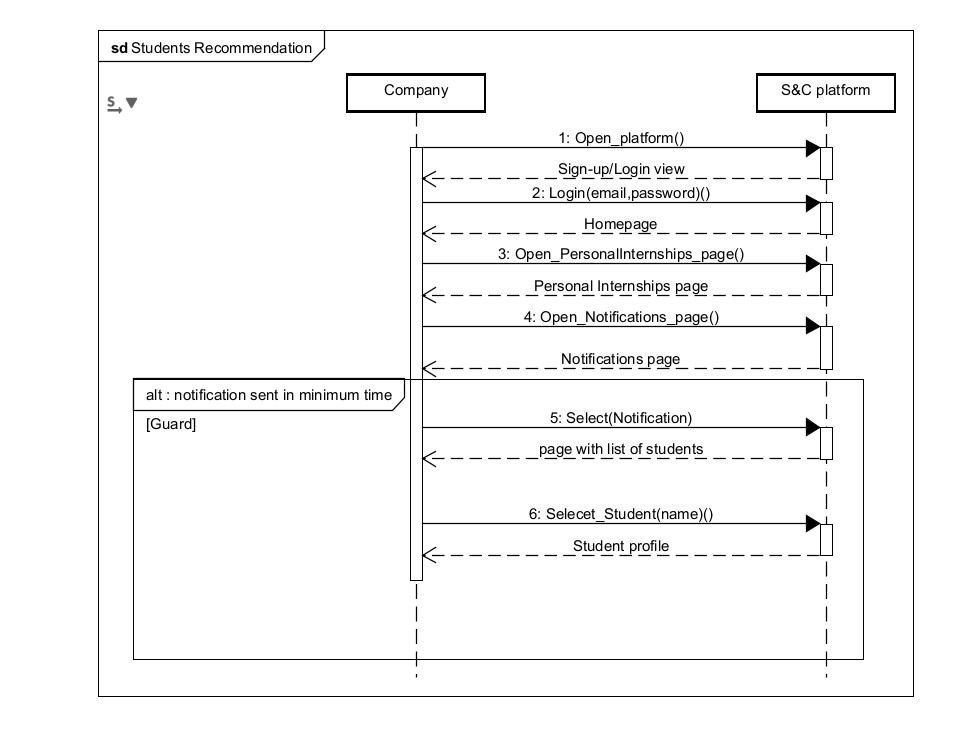
\includegraphics[scale=0.3]{StudentsRecommendation.jpg}
				
			\end{figure}
			
			
			\begin{figure}[H]
				\centering
				{\bfseries [UC10] - Student Application Process}
				\caption{[UC10] - Student Application Process}
				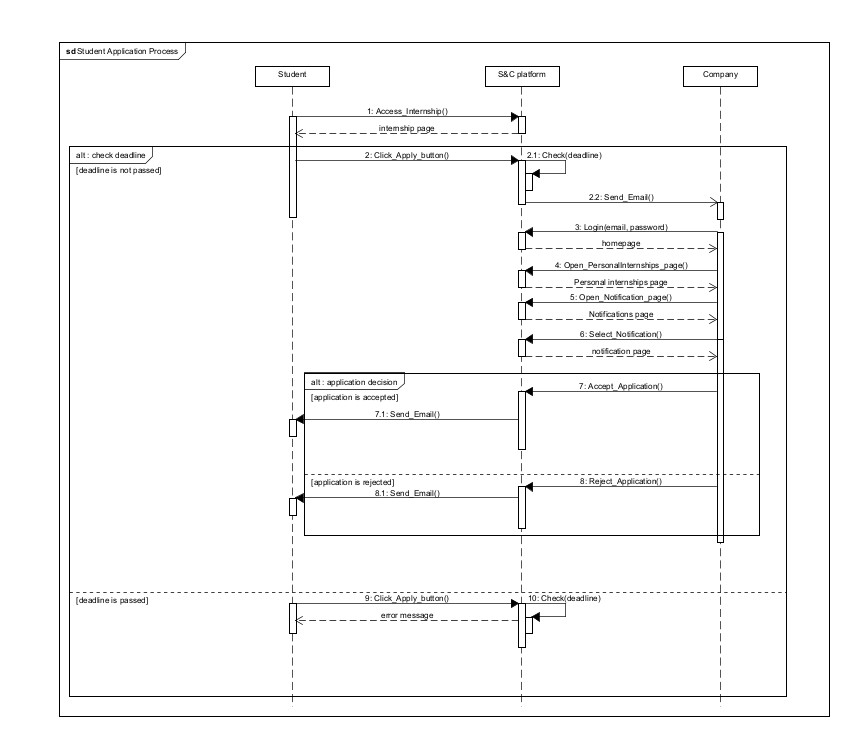
\includegraphics[scale=0.3]{StudentApplicationProcess.jpg}
				
			\end{figure}
			
			\begin{figure}[H]
				\centering
				{\bfseries [UC11] - Company Send of Proposal}
				\caption{[UC11] - Company Send of Proposal}
				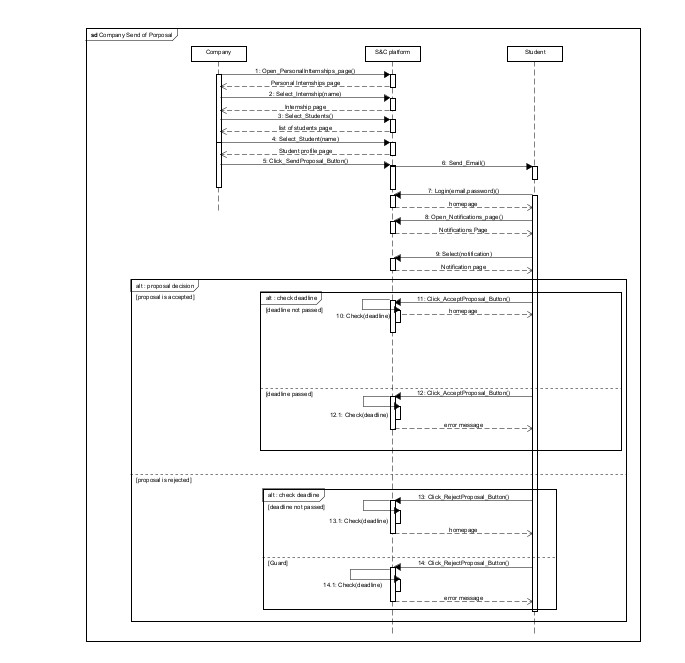
\includegraphics[scale=0.3]{CompanyProposal.jpg}
				
			\end{figure}
			
			\begin{figure}[H]
				\centering
				{\bfseries [UC12] - Selection Process Configuration}
				\caption{[UC12] - Selection Process Configuration}
				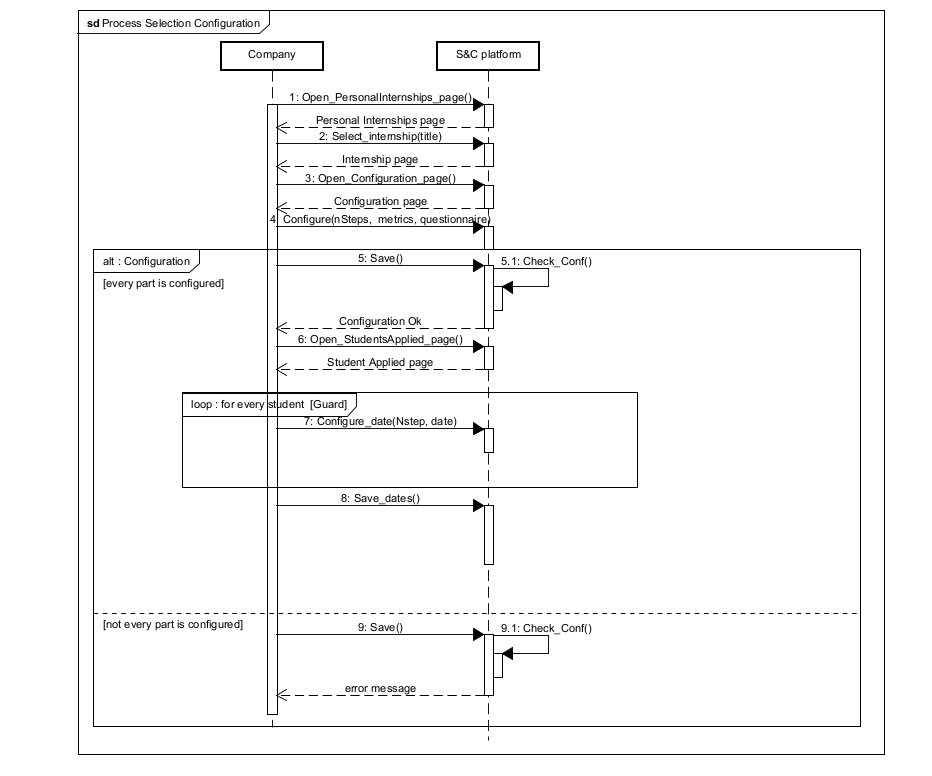
\includegraphics[scale=0.3]{ProcessConfiguration.jpg}
				
			\end{figure}
			
			\begin{figure}[H]
				\centering
				{\bfseries [UC14] - Collection of Student Selection Process Feedback}
				\caption{[UC14] - Collection of Student Selection Process Feedback}
				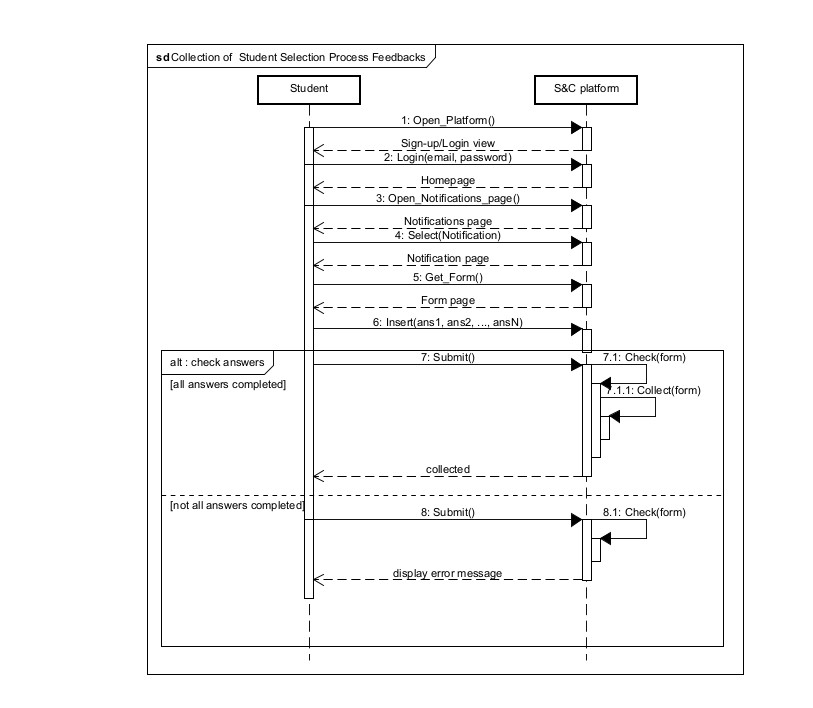
\includegraphics[scale=0.3]{StudentFeedback.jpg}
				
			\end{figure}
			
			\begin{figure}[H]
				\centering
				{\bfseries [UC15] - Collection of Company Selection Process Feedback}
				\caption{[UC15] - Collection of Company Selection Process Feedback}
				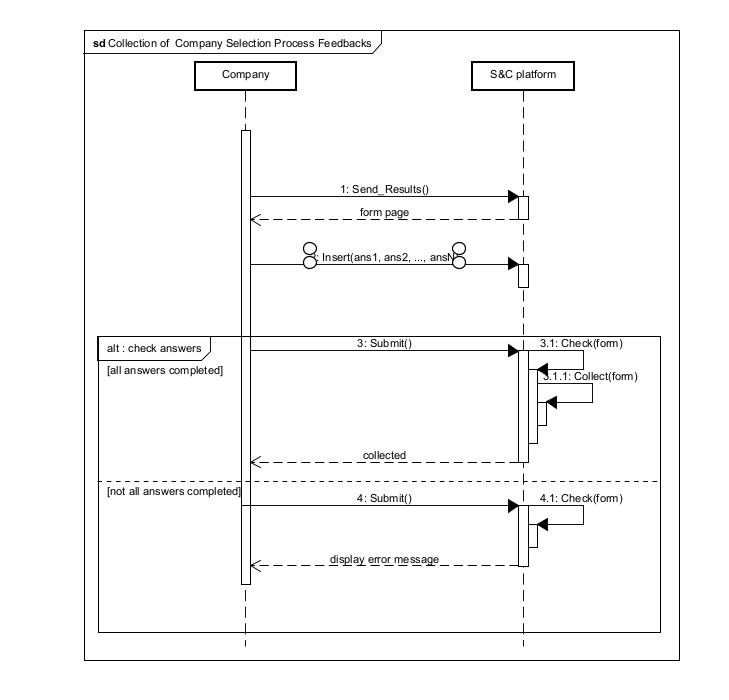
\includegraphics[scale=0.3]{CompanyFeedback.jpg}
				
			\end{figure}
			
			\begin{figure}[H]
				\centering
				{\bfseries [UC16] - Collection of Internships Feedback}
				\caption{[UC16] - Collection of Internships Feedback}
				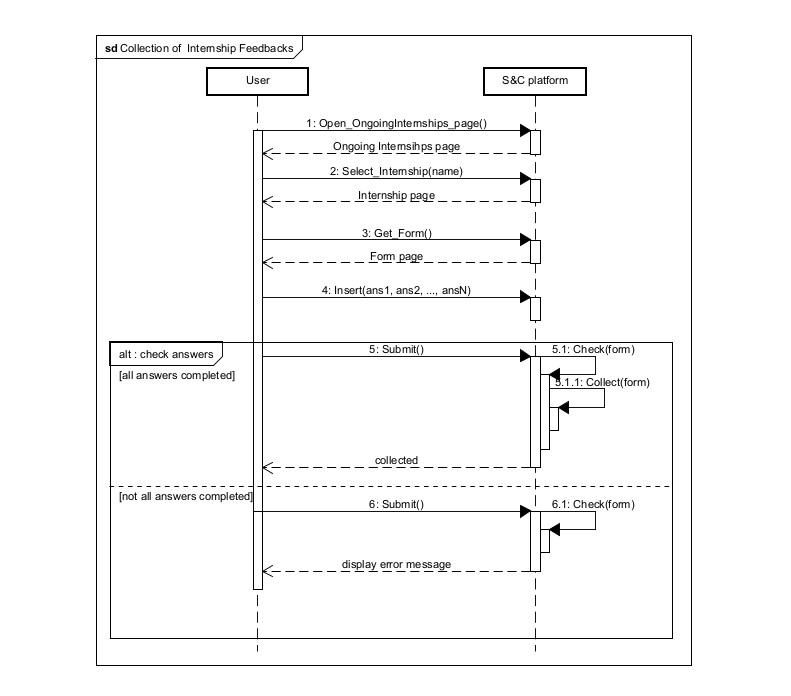
\includegraphics[scale=0.3]{InternshipFeedback.jpg}
				
			\end{figure}
			
			
			\begin{figure}[H]
				\centering
				{\bfseries [UC17] - Collection of Complaints}
				\caption{[UC17] - Collection of Complaints}
				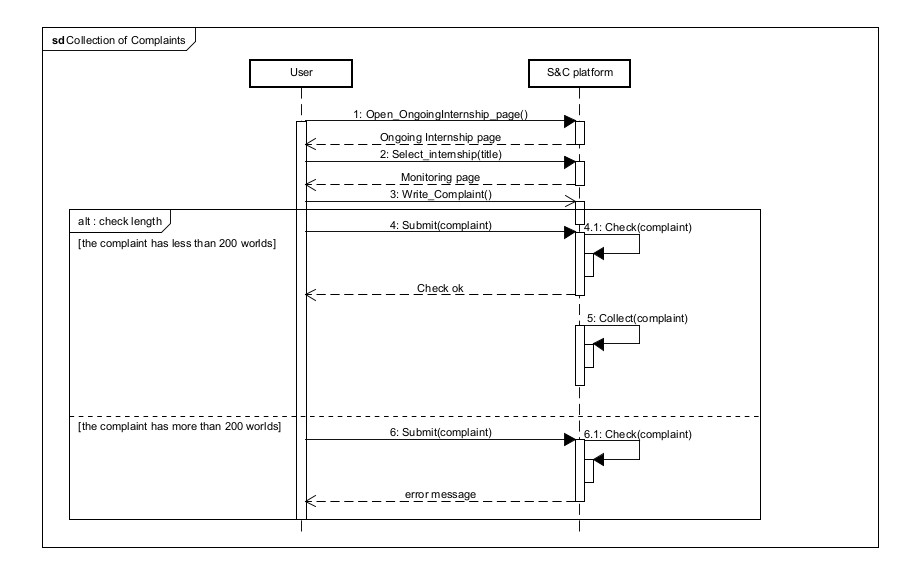
\includegraphics[scale=0.3]{CollectionComplaints.jpg}
				
			\end{figure}
			
			\begin{figure}[H]
				\centering
				{\bfseries [UC18] - Delete Internship Advice}
				\caption{[UC18] - Delete Internship Advice}
				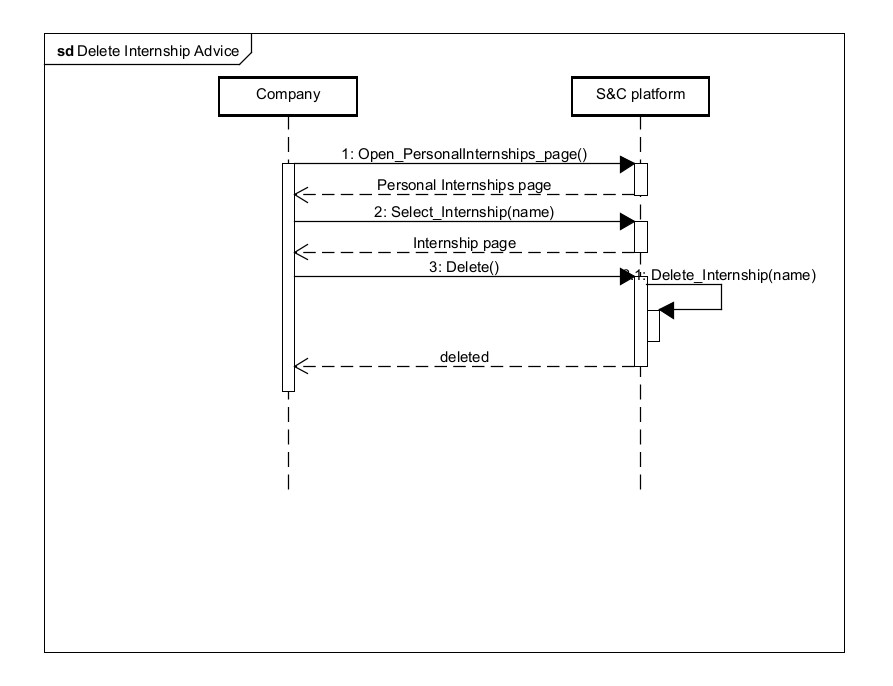
\includegraphics[scale=0.3]{Delete.jpg}
				
			\end{figure}
			
		\subsection{Activity diagrams}
		
			\begin{figure}[H]
				\centering
				{\bfseries [UC13] - Selection process Running}
				\caption{[UC13] - Selection process Running}
				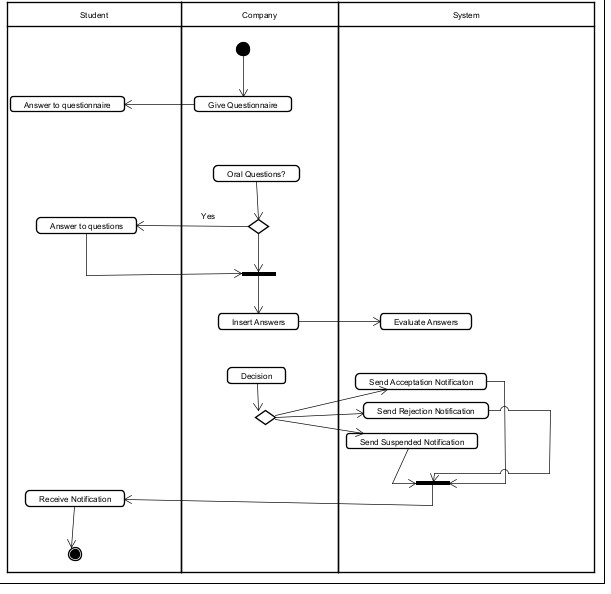
\includegraphics[scale=0.3]{ProcessRun.jpg}
				
			\end{figure}
			
			in the figure it is represented the activity diagram associated do the selection process running UC; in this case we prefer use an activity diagram to represent also the interaction, during the selection interview, between the 2 actors without explicitly using the system; in fact, the filling of the questionnaire and the oral answers are all done without the use of the system; then, to collect the answers, the company use the system and the student receive a notification with the outcome of the interview for this step (Accepted, Rejected, Suspended)
		
	\section{Performance Requirements}
		For the system functions related to user navigation, we require a response time up to 5 seconds.
		
		The mail notification system should send any notification at most 1 minute after the moment in which the notification was generated.
		
		The recommendation system should produce its results with at most 1 week of distance from the last time it produced them.
	\section{Design Constraints}
		\subsection{Standards compliance}
			\begin{itemize}
				\item Since S\&C uses personal data of users, it is necessary that the platform is in compliance with the General Data 		 Protection 	Regulation (GDPR), a regulation in EU law on data protection and privacy for all individuals within the European Union (EU) and the European Economic Area (EEA).
				
				\item The CVs uploaded by students on the platform must necessarily be in the EUROPASS format in order to be processed by the system.
			\end{itemize}
			
		\subsection{Hardware limitations}
		
			To make the best use of the platform, it is necessary that the devices used to access it meet (at least) the following requirements:
			
			\begin{itemize}
				\item\textbf{Internet Connection}: a stable connection of 5 Mbps is required for a smooth experience. This would support navigation on the platform and viewing content. Slower connections may lead to long loading times on pages with a lot of data (note that we don't expect that the application provides large multimedia resources, such as high-quality images or videos);
				\item \textbf{Screen Resolution}: users should have devices with screens of at least 1280x720 px to ensure a good visual experience.
			\end{itemize}
			
		\subsection{Other constraints}
			The platform is designed to allow companies to advertise their internships and for students to find internships relevant to their studies. Therefore, S\&C average users may not have a strong knowledge of UI graphic conventions (e.g. conventional icons), this implies that UI has to be designed in order to meet these usability standards.
	\section{Software System Attributes}
		\subsection{Reliability}
			Considering the criticality of the information managed by the application (e.g. interview dates, CV, e-mail addresses) we require an high level of reliability in each sub-part of the system.
			
			For the recommendation system reliability we ask for a... .
		\subsection{Availability}
			Since the application does not have real-time interactions or much critical functions to ensure, if the system went down for few hours it would not be an huge concern for most users. However, there some functions that require an higher level of availability than the others:
			\begin{itemize}
				\item notification system: it should be available for at least one hour in a day, in order to guarantee that notifications are not sent to users with a delay higher than one day (since notifications are also sent by email, we can rely on the availability of users mail servers, as stated in the assumption section);
				\item selection process system: it is highly recommended that the selections calendars and the relative questionnaires are available at least in work hours. As we stated in the assumption section, we always take for grant the fact that companies (and students) have a copy of calendars (and also of the questionnaires) for the companies;
				\item ongoing internship monitoring: at least in work hours, the monitoring system should be available. Little down-times are still tolerated but it is highly recommended that for the majority of the time is possible to monitor the ongoing internship status.
			\end{itemize}
			As general rule, maintenance should always occur off the work hours of the majority of the companies registered.
		\subsection{Security}
			In this section we define the main kinds of security concern that the system should address:
			\begin{itemize}
				\item e-mails sent from the system always have to be sent from a certified mail address. Moreover, e-mails sent from the system must be encrypted and must not contain any password;
				\item attacks related to system availability (e.g. DOS), to data confidentiality, integrity and users authenticity must be taken into consideration, also considering the public nature of the application;
				\item uploaded CV should be scanned to ensure that they don't contain viruses.
			\end{itemize}
		\subsection{Maintainability}
			For S\&C, which manages multiple users (students and companies) and handles a large amount of sensitive data, maintainability is a crucial aspect:
			\begin{itemize}
				\item the code has to be well documented and tested; in particular, a testing routine has to be provided to check if the system still work or not.
				\item The system structure should provide the ability to deploy updates in the back-end without the users noticing it
				\item to facilitate maintainability, system components should be created to be as modular as possible
			\end{itemize}
		\subsection{Portability}
			We highlight the fact that the application targets are students and companies that may use operative systems of any kind, therefore portability should be increased, in order to spread the audience. On the other hand, non-desktop devices (such as mobile devices, smartwatches ecc.) are not an huge concern of this kind of application, so we don't put much effort on emphasizing the portability also in this direction. At the end, we encourage portability but we ask for it at least for general purposes desktop operative systems.